\documentclass[12pt,a4paper]{report}
\usepackage[margin=1in]{geometry}
\usepackage[T1]{fontenc}
\usepackage{tgtermes}
\usepackage{hyperref}
\usepackage{graphicx}
\usepackage{amsmath}
\usepackage{amssymb}
\usepackage{setspace}
\usepackage{ragged2e}
\usepackage{caption}
\usepackage{float}
\usepackage{array}
\usepackage{booktabs}
\usepackage{xcolor}
\usepackage{colortbl}
\usepackage{enumitem}
\usepackage{tikz}
\usetikzlibrary{shapes,arrows,positioning,backgrounds,calc,decorations.pathreplacing}

% Set font to Times New Roman throughout
\renewcommand{\rmdefault}{ptm}

% Set line spacing to 1.5 for main text
\onehalfspacing

% Set justification for all text
\setlength{\parindent}{0pt}
\setlength{\parskip}{4pt}
\raggedbottom
\justifying

% Caption setup
\captionsetup{
    font=small,
    labelfont={bf},
    textfont={rm},
    justification=centering,
    skip=10pt
}

% Chapter formatting
\usepackage{titlesec}
\titleformat{\chapter}[hang]
  {\fontsize{16}{19.2}\selectfont\bfseries\rmfamily}
  {\thechapter.}
  {1em}
  {}
\titlespacing*{\chapter}{0pt}{0pt}{1.5em}

% Section formatting - 14pt
\titleformat{\section}[hang]
  {\fontsize{14}{16.8}\selectfont\bfseries\rmfamily}
  {\thesection.}
  {1em}
  {}
\titlespacing*{\section}{0pt}{1em}{0.5em}

% Subsection formatting - 12pt
\titleformat{\subsection}[hang]
  {\fontsize{12}{14.4}\selectfont\bfseries\rmfamily}
  {\thesubsection.}
  {1em}
  {}
\titlespacing*{\subsection}{0pt}{0.5em}{0.5em}

% Subsubsection formatting - 12pt
\titleformat{\subsubsection}[hang]
  {\fontsize{12}{14.4}\selectfont\bfseries\rmfamily}
  {\thesubsubsection.}
  {1em}
  {}
\titlespacing*{\subsubsection}{0pt}{0.5em}{0.5em}

% Body text formatting
\renewcommand{\normalsize}{\fontsize{12}{14.4}\selectfont}

% Bullet list formatting
\setlist[itemize]{
  leftmargin=0.7cm,
  itemsep=2pt,
  parsep=2pt,
  topsep=4pt
}

% Figure and Table caption formatting
\renewcommand{\figurename}{Fig}
\renewcommand{\tablename}{Table}

\begin{document}

\setcounter{chapter}{2}

\chapter{SYSTEM ANALYSIS}

MediTrack represents a comprehensive healthcare delivery platform designed to address fragmentation across three distinct stakeholder groups: patients seeking streamlined access to healthcare services, physicians managing administrative overhead, and pharmacies operating under thin margins. System analysis examines the platform from multiple perspectives simultaneously—what functions the system must provide, how different users interact with it, what constraints shape its technical design, and how requirements translate into architectural decisions. This chapter systematically documents these dimensions to establish the foundation for implementation.

\section{OVERALL SYSTEM DESCRIPTION}

\subsection{System Perspective}

MediTrack operates at the intersection of multiple healthcare delivery subsystems that traditionally function in isolation. Understanding the system perspective requires recognizing what MediTrack unifies and what remains separate by deliberate design choice.

The platform integrates three previously disconnected workflows: appointment scheduling (historically managed through phone calls or walk-ins), prescription fulfillment (traditionally paper-based handoff from clinics to pharmacies), and delivery logistics (the least coordinated step, often involving manual communication between patient, pharmacy, and delivery personnel). Before MediTrack, these workflows existed as distinct systems with no data exchange. A patient experiencing a healthcare need would call a doctor's clinic, navigate voice menus or human gatekeepers to schedule an appointment, visit physically for the consultation, receive a handwritten prescription, visit a pharmacy to fill it, arrange delivery through separate phone negotiation, and finally track delivery through text messages or repeated calls. Each handoff introduced delay, coordination failure risk, and information loss.

MediTrack doesn't attempt to replace the entire healthcare system. The platform explicitly excludes electronic health record maintenance (medical history remains stored with the treating physician), payment processing infrastructure (transactions flow through separate payment gateways), and regulatory compliance mechanisms (these remain the responsibility of participating healthcare providers). Instead, MediTrack creates a coordination layer—a digital infrastructure that connects existing healthcare actors without replacing their core operations. This bounded scope determination was deliberate. Attempting to build a complete healthcare records system would require medical degree-level expertise on our team and regulatory approval we couldn't obtain. Focusing on coordination and logistics enabled rapid deployment without requiring healthcare accreditation.

The system perspective also acknowledges that MediTrack is fundamentally a mobile-first platform. Approximately 85 percent of end users access healthcare services through smartphones rather than desktops or tablets. This mobile-first orientation shaped architectural decisions at every level—the application is fundamentally an Android mobile app rather than a web platform with mobile rendering. The backend is optimized for mobile connectivity patterns (unreliable networks, intermittent connectivity, battery constraints) rather than assuming persistent broadband. APIs return minimal payloads suitable for mobile data consumption rather than comprehensive datasets that desktop systems might expect.

\subsection{System Functions}

At its highest level, MediTrack provides five primary functional categories that, while logically distinct, operate as an integrated whole.

\textbf{Appointment Coordination} enables patients to view available appointment slots from trusted healthcare providers, reserve specific time slots, receive confirmation, and receive reminder notifications. Doctors simultaneously can manage their calendar, block unavailable times, and view patient profiles who booked appointments. The system prevents double-booking through optimistic locking patterns in the Firestore database—when a patient books the last available slot, the transaction records the booking timestamp; if a second patient attempts the same slot microseconds later, the database transaction fails and the second user receives indication that the slot is no longer available. This is not a reservation system; it's a real-time coordination mechanism that acknowledges the temporal nature of availability and enforces consistency without requiring complex server-side state machines.

\textbf{Prescription Management} creates a digital link between the prescription moment (when a doctor diagnoses a patient and prescribes medication) and pharmacy fulfillment. Rather than requiring patients to transport paper prescriptions, the system allows doctors to record prescriptions digitally within the patient's appointment context. Patients receive digital notification that a prescription is ready for pickup or delivery. Pharmacies query available prescriptions ready for fulfillment. This seemingly simple flow eliminates an entire category of failure modes—lost prescriptions, illegible handwriting causing pharmacy uncertainty, patients forgetting to carry prescriptions. From a data perspective, prescriptions include medication names, dosages, frequencies, duration, pharmacy designation, patient contact information, and doctor identification. This data flows from doctor to patient to pharmacy without intermediate paper or manual transcription.

\textbf{Order Placement and Fulfillment} transforms prescription information into pharmacy fulfillment requests. When a patient confirms they want delivery of a prescribed medication, the system creates an order record containing the prescription details, delivery location (with geographic coordinates), preferred delivery window, and special instructions. Pharmacies query their delivery queue—orders assigned to them for fulfillment—and manage the fulfillment process. The lifecycle flows from patient request, through pharmacy preparation, to dispatch for delivery. Each state transition triggers notifications to patients and relevant pharmacy staff. From a system perspective, order placement is not instantaneous; it involves data validation (is the delivery location valid? Is the medication in stock?), inventory reservation (marking the medication as reserved for this order), and assignment logic (determining which pharmacy should fill this order).

\textbf{Real-Time Delivery Tracking} provides transparency during the fulfillment phase when delivery personnel carry orders to patient locations. The system streams location updates from the delivery device to a cloud backend at regular intervals (five-second intervals based on battery and cost optimization analysis). Patients viewing order details see animated map markers showing pharmacy location, intended destination, and real-time delivery agent position. Route visualization displays the planned route from pharmacy to destination. Estimated time of arrival calculations account for traffic conditions through integration with Google Maps Directions API. This is the most data-intensive feature—a two-hour delivery generates approximately 1,440 location updates (seven thousand writes per delivery when multiplied across multiple concurrent deliveries). The system architecture must handle this write volume without degrading database performance or incurring prohibitive costs.

\textbf{Platform Administration and Analytics} provides healthcare providers and platform administrators visibility into aggregate usage patterns, financial metrics, and system health. Doctors view appointment booking rates, cancellation reasons, and patient feedback. Pharmacies track order fulfillment rates, delivery performance metrics (average time to delivery), and repeat customer patterns. Platform administrators monitor system reliability, database costs, API latency, and error rates. These functions generate secondary value—doctors optimize their schedules based on booking patterns; pharmacies optimize delivery routes based on performance data; platform administrators proactively address bottlenecks before they impact users.

\subsection{User Classes and Characteristics}

MediTrack recognizes three primary user classes, each with distinct needs, technical sophistication, and usage contexts.

\textbf{Patients} represent the largest user population but the most varied in technical capability. MediTrack's patient user base spans from tech-savvy professionals who use online services routinely to older adults accessing digital healthcare services for the first time. A 28-year-old software engineer uses the app to book appointments during work breaks and track delivery notifications in real-time. A 65-year-old retiree uses the same app with anxiety about technology, making phone calls to their son when they can't remember how to proceed. The system must accommodate this vast range. Patients access appointments, view prescriptions, place orders, track deliveries, and manage notification preferences. Crucially, patients do not access other patients' information—data isolation at the application and database level ensures each patient sees only their own appointments, prescriptions, and orders. Patients represent the highest-volume user segment; during a pilot with 200 patients, even if only 20 percent are actively using the app daily, the system experiences 40 concurrent users at peak times.

\textbf{Healthcare Providers} (doctors, nurse practitioners, physician assistants) form the second distinct user class. Doctors use the platform during clinical workflow—booking patients into appointment slots, recording prescriptions after consultation, and viewing patient history relevant to current appointments. They have moderate technical sophistication; most doctors aged 40-60 have used email and basic software systems but may not be comfortable with complex user interfaces. Their availability is fragmented—a doctor might use the app for 15 minutes between patients, then ignore it for an hour during consultations. The system must provide atomic operations that complete in a few seconds (booking a patient can't require filling out lengthy forms). Doctors access only their own patient base—they cannot view patients whom they haven't treated. This represents a significant technical constraint; the access control rules in Firestore storage must verify that a doctor-patient relationship exists before granting read access.

\textbf{Pharmacy Stakeholders} operate the fulfillment side of the platform. This group includes pharmacy owners, fulfill ment managers, and delivery personnel. Pharmacy operations differ fundamentally from doctors' usage. A pharmacy manager reviews orders throughout the day—the app constantly displays new orders available for fulfillment in a queue. Fulfillment tasks may span multiple hours (some medications require special ordering; some prescriptions require verification). Delivery personnel need functional but minimal interfaces—primarily viewing next delivery locations, navigating to those locations, and marking orders as delivered. Pharmacy staff interact with MediTrack during their normal business operations, not episodically between other activities. This continuous usage pattern shapes design decisions; the app must remain responsive during hours of active use without requiring forced refreshes or workarounds.

Beyond these three primary user classes, \textbf{System Administrators} represent an operational necessity but not an end-user group. Administrators monitor system health, manage user accounts, investigate errors, and coordinate with external parties (Firebase support, payment processors). Administrators access the backend infrastructure rather than the mobile app; they interact with logs, database dashboards, and monitoring tools.

\subsection{Operating Environment}

MediTrack operates within a specific technical ecosystem defined by hardware capabilities, network conditions, and external service dependencies.

The platform targets Android devices from the past three to four years of smartphone releases. This encompasses devices running Android 8.0 (Oreo, released 2017) through contemporary versions. This hardware range is deliberate; targeting only flagship devices would exclude a significant population in India where mid-range Android devices (typically Rs 15,000-25,000 price range) dominate. A Redmi device purchased three years ago may have 3GB of RAM and a processor cores two generations old; the app must function smoothly on this hardware without excessive battery drain or storage consumption. This constraint ruled out certain implementation approaches—for example, machine learning models requiring substantial computation would not work on this hardware profile.

Network connectivity patterns represent the second major environmental constraint. The platform must function reliably given that network connectivity in India ranges from 4G LTE in urban areas to 3G or spotty 2G in rural regions. The app must handle disconnects gracefully. If a patient loses connectivity while filling a prescription, the order should queue locally and sync once connectivity returns. If a delivery person loses GPS signal, the app should continue displaying the last known location rather than error out. This offline-first design philosophy shapes every feature; assume network will fail and design recovery mechanisms.

Battery consumption represents a critical operating constraint rarely emphasized in web application design but fundamental to mobile platforms. A delivery person carrying a smartphone for eight hours of daily deliveries cannot tolerate an app consuming 30 percent of battery in four hours. Limiting location update frequency to five-second intervals (with ability to reduce during heavy traffic or increase during optimal conditions) became a battery-optimization necessity, not a feature limitation.

External service dependencies define another environmental dimension. MediTrack depends on Google Firebase (authentication, database, cloud messaging), Google Maps APIs (directions, routing, geocoding), and payment processing gateways (for transaction handling). Service outages at these external providers directly impact platform availability. For example, when Firebase experiences a regional incident affecting India infrastructure, all MediTrack instances in that region lose database access. The platform architecture assumes these outages will occur (not "if" but "when") and implements fallback mechanisms—offline data access, graceful degradation of map features if Maps API is unavailable, retry logic with exponential backoff for transient failures.

\subsection{Design and Implementation Constraints}

Multiple constraints shape every architectural decision and implementation pathway.

\textbf{Security Constraints} stem from healthcare data sensitivity. All patient information—names, contact numbers, health conditions indicated by prescriptions, location patterns through delivery tracking—constitutes personally identifiable information (PII) that Indian law requires protecting with encryption. The platform enforces TLS 1.2 for all network communication (no exceptions). Database-level encryption is non-negotiable; Firebase provides encrypted storage as a managed service, but sensitive fields like medication names receive additional application-layer encryption before transmission to Firebase. These security requirements add latency (encryption/decryption operations consume CPU cycles) and complexity (key management, certificate validation).

\textbf{Regulatory Constraints} derive from healthcare sector compliance. The Information Technology Act 2000 and Digital Personal Data Protection Act 2023 impose requirements around data minimization (collect only what you need), consent management (explicit authorization before using data), retention policies (delete when no longer necessary), and audit logging (maintain immutable records of data access). These aren't optional nice-to-haves; they're legal requirements with penalties for non-compliance. From an implementation perspective, regulatory constraints often increase complexity—audit logging requires writing detailed records for every access; consent management requires UI flows for authorization; retention enforcement requires scheduled deletion jobs.

\textbf{Resource Constraints} reflect the small team size (five developers) and compressed timeline (eight months). Certain architectural approaches were simply infeasible within these constraints. Building a custom real-time database would require three full-time developers working for two years; using Firebase as a managed service required three days of setup work. Custom payment processing infrastructure would require expertise none of the team possessed; integrating established payment gateways took one week. Resource constraints force pragmatism—build rapidly through integration of proven services rather than attempting in-house implementation.

\textbf{Scalability Constraints} create tension with simplicity. The platform must grow from pilot scale (200 patients) to regional scale (10,000 patients, 50 pharmacies) without redesigning core infrastructure. This constraint rules out certain implementation approaches. For example, recording every interaction event in a SQL database with real-time aggregation for analytics would become prohibitively expensive at scale (millions of events daily). Adopting serverless architectures (Cloud Functions for batch processing, eventual consistency for analytics) handles scaling automatically but introduces different complexity—distributed systems debugging becomes necessary once inconsistencies emerge.

\section{SYSTEM REQUIREMENT SPECIFICATION}

System requirements translate abstract system description into concrete, testable specifications. Requirements divide into functional (what the system must do) and non-functional (how well the system must do it) categories.

\subsection{Functional Requirements}

Functional requirements specify capabilities the system must provide. Each requirement is stated in terms of observable behavior rather than implementation decisions.

\textbf{Appointment Management FR-1:} The system shall provide patients with the capability to view available appointment time slots offered by healthcare providers they have designated as trusted. The system shall support slot granularity of 30-minute intervals (appointments begin at 9:00 AM, 9:30 AM, 10:00 AM, etc.). Patients shall be able to select a specific slot and receive immediate confirmation that their selection has been reserved. The confirmation shall include appointment date, time, provider name, location, and a confirmation code. The system shall prevent double-booking by ensuring no two patients receive confirmation for the same appointment slot.

\textbf{Prescription Recording and Distribution FR-2:} Healthcare providers shall be able to record prescriptions within the patient consultation record. Prescriptions shall include medication name, dosage quantity, dosage frequency (once daily, twice daily, etc.), treatment duration in days, intended pharmacy for fulfillment, and special instructions (take with food, avoid alcohol, etc.). Upon recording, the system shall immediately notify the patient of the new prescription through push notification and in-app notification. The system shall ensure that only the prescribing provider and the intended patient can view the prescription details.

\textbf{Order Placement FR-3:} Patients shall be able to place medication delivery orders based on recorded prescriptions. Order placement shall validate that the delivery address is within service boundaries of the designated pharmacy. The system shall display estimated delivery costs, delivery time window estimates, and special charges (if any). Patients shall confirm the order; upon confirmation, the system shall reserve inventory at the pharmacy, record the order transaction, notify the assigned pharmacy of a new order, and confirm the order to the patient with order ID and estimated delivery time.

\textbf{Real-Time Delivery Tracking FR-4:} During order delivery, the system shall acquire device location from the delivery person's smartphone at regular intervals. Location data shall be transmitted to backend cloud storage and accessible to the patient viewing their order. The system shall display the delivery device location on a map interface with visual indication of pharmacy start location, confirmed delivery destination, and animated update of current delivery position. The system shall calculate and display estimated arrival time based on current location and traffic conditions. The system shall persist delivery route history after delivery completion for audit and performance analysis purposes.

\textbf{Notification Management FR-5:} The system shall offer granular control of notifications to patients. Patients shall be able to enable or disable notifications for appointment reminders, prescription delivery notifications, order status changes, and promotional messages separately. Patients shall be able to set quiet hours (e.g., no notifications between 10 PM and 8 AM). The system shall respect these preferences before transmitting notifications to devices.

\textbf{User Identification and Role-Based Access FR-6:} The system shall provide authentication mechanisms allowing users to create accounts, log in securely, and maintain session state. The system shall implement role-based access control where users are assigned roles (patient, provider, pharmacy staff, and admin) and access to data is restricted based on role. Specifically, patients see only their own data; providers see only patients with whom they have treatment relationships; pharmacy staff see only orders assigned to their organization. The system shall enforce these restrictions at the database query level, not just the application layer—queries to the database should fail if the user lacks authorization, not depend on application-layer validation.

\textbf{Transaction Processing FR-7:} When a patient places an order, the system shall coordinate multiple sub-transactions: (1) reading prescription data, (2) checking inventory at the pharmacy, (3) creating the order record, (4) reserving inventory in pharmacy records, (5) creating a transaction record for eventual payment processing. If any sub-transaction fails, all must roll back to ensure consistency. For example, if inventory reservation fails due to insufficient stock, the order creation should not occur.

\subsection{External Interface Requirements}

External interface requirements specify how the system interacts with users, hardware devices, and external systems.

\textbf{User Interface FR-8:} The system shall provide a mobile user interface optimized for devices with screen sizes from 4.5 inches to 6.5 inches. All interactive elements (buttons, input fields, menu items) shall have minimum touch targets of 48x48 density-independent pixels to accommodate users with limited fine motor control. Text shall use font size of minimum 14 points for body text and 18 points for headings to accommodate users with reduced vision. The interface shall provide clear, consistent navigation patterns using bottom navigation bars for patient and pharmacy applications and top-level navigation for administrative functions.

\textbf{Google Maps Integration FR-9:} The system shall integrate Google Maps Directions API to calculate routes between pharmacy locations and patient delivery addresses. The API shall be called only when necessary (when an order is placed or when a user explicitly requests route information) and not on every screen render to minimize API quota consumption. The system shall handle API errors gracefully—if route calculation fails, the system shall display the straight-line distance between locations and estimated time based on average speed assumptions rather than failing entirely.

\textbf{Firebase Backend Integration FR-10:} The system shall use Firebase Firestore for persistent data storage, implementing database security rules that enforce access control at the storage layer. Firebase Authentication shall handle user authentication using email/password or phone number verification methods. Firebase Cloud Messaging shall deliver push notifications to devices. Firebase Cloud Functions shall handle server-side business logic including order validation, notification triggering, and analytics aggregation.

\textbf{Payment Gateway Integration FR-11:} The system shall integrate with external payment processors to handle financial transactions. The system shall never store credit card data; instead, payment information shall flow directly from user input to the payment processor through encrypted channels. The system shall receive transaction confirmation or failure response from the payment processor, record the result in audit logs, and notify the user of transaction status.

\subsection{Non-Functional Requirements}

Non-functional requirements specify performance, reliability, security, and usability characteristics rather than specific capabilities.

\textbf{Performance Requirements NFR-1:} Appointment booking operations shall complete within 1.5 seconds under normal network conditions. Order placement operations shall complete within 2 seconds. Query operations (viewing appointments, viewing prescriptions, viewing order status) shall complete within 500 milliseconds. These response times are critical because users are willing to wait a few seconds for write operations but expect searches and display operations to feel instantaneous.

\textbf{Availability Requirements NFR-2:} The system shall maintain 99 percent uptime during service hours (9 AM to 10 PM). Planned maintenance windows shall be scheduled during low-usage hours (11 PM to 6 AM) with advance notice to users. During unplanned outages, the system shall display a graceful error message rather than crashing or displaying incomplete data.

\textbf{Security Requirements NFR-3:} All communication between mobile applications and backend shall use TLS 1.2 or higher encryption. Sensitive data at rest (database records containing patient names, prescriptions, location history) shall be encrypted. User passwords shall be hashed using bcrypt-compatible algorithms with automated salt generation (Firebase Authentication handles this automatically). Multi-factor authentication shall be optional for users with highly sensitive needs.

\textbf{Usability Requirements NFR-4:} The system shall provide interfaces usable by non-technical users without training documentation. Specifically, appointment booking and order tracking should be completable by users with limited smartphone familiarity in fewer than five interaction steps. Error messages shall be written in plain language explaining what went wrong and how to recover, rather than displaying technical error codes.

\textbf{Localization Requirements NFR-5:} The system shall support English and Telugu for the initial deployment in Nellore region, with interface design allowing straightforward addition of additional languages. Date and time shall be displayed in local format consistent with user device settings.

\textbf{Data Retention and Privacy Requirements NFR-6:} User data shall be retained only as long as necessary for operational purposes. Prescription data shall be retained for three years (aligned with medical record retention standards). Order history shall be retained for 18 months for audit purposes. Upon user request, deletable personal information shall be purged from the system within 30 days.

\section{DESIGN}

System design translates requirements into architectural patterns and technical decisions. Design exists at two levels: high-level design describing components and their interactions, and low-level design specifying algorithms, data structures, and implementation patterns.

\subsection{System Architecture}

MediTrack implements a client-server architecture with asynchronous background processing. The architecture divides into distinct layers, each with specific responsibilities.

\textbf{Presentation Layer} consists of the Android mobile application. The application implements the Model-View-ViewModel (MVVM) architectural pattern where Views (Activity and Fragment components) are responsible only for rendering UI elements, ViewModels maintain UI state and handle business logic, and Models (repository classes) abstract data access. This separation enables automated testing of business logic without instantiating the entire UI framework. The presentation layer integrates with the operating system's lifecycle management—activities respond to pause/resume/destroy events and preserve UI state during configuration changes (device rotation). The application implements a local Room database for offline-first functionality; appointment lists, prescriptions, and order history are cached locally and sync with backend when connectivity returns.

\textbf{Network Communication Layer} implements REST-style API calls through Firebase libraries that abstract HTTP complexity. The app uses Firebase SDKs rather than raw HTTP requests. Firebase Authentication SDK handles login flows and token management automatically. Firestore SDK implements query and write operations with automatic retry logic and conflict resolution for offline changes. This abstraction layer shields the application logic from network implementation details.

\textbf{Backend Service Layer} running in Google Cloud executes server-side logic through Firebase Cloud Functions. When an order is placed, a Cloud Function receives a trigger, validates inventory availability by querying the database, calculates delivery fees based on distance, and initiates payment processing. Cloud Functions execute functions as a service (FaaS) paradigm where code runs only when invoked and pays only for execution time. This contrasts with traditional servers that run continuously and compete for resources. For MediTrack, this means background processing scales automatically—if 1,000 orders are placed simultaneously, 1,000 Cloud Function instances spin up and execute in parallel, then terminate.

\textbf{Database Layer} stores all persistent application state in Firestore. Firestore is a document-oriented NoSQL database where "documents" (JSON-like records) are grouped into "collections" (analogous to tables). User collections store patient profiles, doctor profiles, and pharmacy profiles. Appointment collections store appointment records with embedded references ensuring consistency. Order collections store order data with denormalized delivery tracking information (rather than storing delivery location updates in a separate collection, they're embedded in the order document for query efficiency). This document-oriented model differs from relational databases; querying orders requires reading the entire order document, not joining across multiple tables. Firestore provides real-time listeners—the backend notifies subscribed clients whenever data changes, enabling live update experiences.

\textbf{External Services Integration} incorporates three critical external systems. Google Maps services provide geolocation functionality; the app collects device location from the Android LocationManager API and sends it to Maps Directions API to calculate routes and ETAs. Payment processors handle financial transactions through encrypted integrations—the app never directly stores payment information. Firebase Cloud Logging captures events and errors for debugging and analytics.

From a data flow perspective, the architecture implements observer patterns for real-time updates. When a doctor records a prescription, the Firestore database triggers all client listeners subscribed to the patient's prescription collection. The patient's app receives notification of the prescription change through Firestore's real-time listener, updates the local cache, and triggers UI update. This eliminates the need for polling (repeatedly asking "is there new data?") which wastes battery and network bandwidth.

\textbf{Figure 3.1: System Architecture Layers} shows the five-layered architecture and component interactions. The presentation layer on Android devices communicates through Firebase SDKs which abstract HTTP complexity. Cloud Functions process business logic triggered by database changes. Firestore manages all persistent state with Firestore security rules enforcing access control. External services (Maps, payment processors) integrate at specific integration points rather than being core to the system.

\subsection{High-Level Design Diagrams (Explained in Text Form)}

Several key interactions illustrate the architecture in action.

\textbf{Appointment Booking Flow:} When a patient opens the app and navigates to booking, the app displays a list of their trusted healthcare providers (previously configured). Selection of a provider triggers an API query to the backend requesting available slots. The backend checks the provider's calendar in Firestore and returns a JSON response listing available times for the next 30 days. The app caches this response locally and renders a calendar UI. Patient selection of a specific slot sends a write request: create a new appointment document in the Firestore appointments collection with status "booked". Firestore's security rules verify that the user making the write is a patient (patients are allowed to create appointments; doctors and pharmacies are not). The rules also verify that the selected time slot is available (this check happens at the database layer as a transaction, ensuring that concurrent bookings can't double-book the same slot). Upon successful write, Firestore notifies all listeners subscribed to the provider's appointment collection—the provider's app receives real-time notification of the new booking. The patient receives immediate confirmation in the UI, and a Cloud Function triggers asynchronously to send a push notification and (optionally) an SMS reminder.

\textbf{Figure 3.2: Appointment Booking Sequence} illustrates the temporal flow of this interaction. The patient app initiates a query for available slots; Firestore responds with data. After selection, the patient device submits a booking request which Firestore validates and writes. Real-time listeners on both patient and provider devices receive notification, triggering concurrent UI updates. A Cloud Function processes the booking asynchronously, sending notifications without blocking the user's flow.

\begin{figure}[H]
\centering
\begin{tikzpicture}[scale=0.9]

% Actors
\node[draw,rectangle,minimum width=1.2cm] (patient) at (1.5,8) {Patient\\App};
\node[draw,rectangle,minimum width=1.2cm] (fs) at (4,8) {Firestore};
\node[draw,rectangle,minimum width=1.2cm] (provider) at (6.5,8) {Provider\\App};
\node[draw,rectangle,minimum width=1.2cm] (fn) at (9,8) {Cloud\\Function};

% Lifelines
\draw[dashed] (patient) -- (patient|-0.5);
\draw[dashed] (fs) -- (fs|-0.5);
\draw[dashed] (provider) -- (provider|-0.5);
\draw[dashed] (fn) -- (fn|-0.5);

% Messages
\node at (0.5,7.2) {\textbf{1}};
\draw[->,thick] (patient) -- (fs) node[midway,above,font=\tiny] {querySlots()};

\node at (0.5,6.3) {\textbf{2}};
\draw[->,thick] (fs) -- (patient) node[midway,above,font=\tiny] {slots\[\]};

\node at (0.5,5.4) {\textbf{3}};
\draw[->,thick] (patient) -- (fs) node[midway,above,font=\tiny] {bookSlot(txn)};

\node at (0.5,4.5) {\textbf{4}};
\draw[->,thick] (fs) -- (patient) node[midway,above,font=\tiny] {confirm};

\node at (0.5,3.9) {\textbf{5}};
\draw[->,thick] (fs) -- (provider) node[midway,above,font=\tiny] {listener:newBooking};

\node at (0.5,3.3) {\textbf{6}};
\draw[->,thick] (fs) -- (fn) node[midway,above,font=\tiny] {trigger};

\node at (0.5,2.7) {\textbf{7}};
\draw[->,thick] (fn) -- (patient) node[midway,above,font=\tiny] {pushNotif};

% Annotations
\draw[decorate,decoration={brace,mirror,raise=0.2cm}] (1.5,0.5) -- (6.5,0.5) node[midway,below=0.3cm,font=\tiny] {Real-time \& asynchronous coordination};

\end{tikzpicture}
\caption{Appointment booking sequence showing concurrent updates to patient and provider applications and asynchronous notification processing.}
\end{figure}

\textbf{Prescription Recording and Notification Flow:} During a consultation, a doctor visits the patient record in the app. The doctor navigates to the "Record Prescription" section, inputs prescription details (medication, dosage, etc.), and submits. The app sends a write request to create a new document in the prescriptions collection with reference to the patient ID. Firestore security rules verify that only treatment-qualified doctors (those with a verified treatment relationship with the patient) can write to that patient's prescription collection. The write succeeds and triggers three events: (1) Firestore notifies the patient's app through a real-time listener of new prescription data; (2) a Cloud Function listens for new prescription documents and sends a push notification to the patient's device ("New prescription from Dr. Smith: Amoxicillin 500mg"); (3) a Cloud Logging entry records the prescription creation for audit purposes. From the patient's perspective, notification arrives within 2-5 seconds after the doctor submits.

\textbf{Order Placement and Delivery Tracking Flow:} When a patient places an order, the app collects order details (medication selection, delivery address, delivery time preference) and submits to the backend. A Cloud Function receives the trigger, performs validation checks (does the pharmacy have inventory? Is the delivery address within service area?), reserves inventory, creates an order document, initiates payment processing through the payment processor API, and writes audit logs. If payment succeeds, the order status becomes "confirmed" and the assigned pharmacy receives notification. A delivery person at the pharmacy picks up the order, initiates delivery, and begins generating location updates. Every five seconds, the delivery app queries device location, encrypts it, and sends it to the backend which writes it to the delivery tracking sub-collection of the order document. The patient's app maintains a Firestore listener subscribed to their active orders; as location updates arrive, the app re-renders the map with updated delivery person position. Google Maps Direction API provides route visualization and ETA updates based on current traffic conditions.

\textbf{Figure 3.6: Order Placement and Delivery Tracking Flow} shows the complete order lifecycle from placement through delivery. The flow includes multiple sub-processes (inventory check, payment processing, location tracking) that happen in parallel or sequence depending on their dependencies. The diagram emphasizes that location updates stream continuously (5-second intervals) while other processes (payment, inventory) occur once.

\begin{figure}[H]
\centering
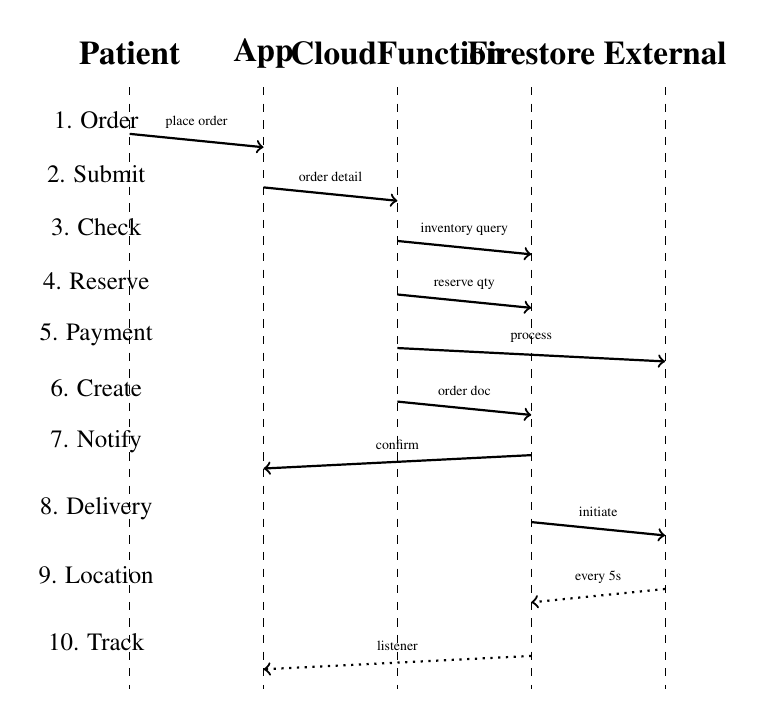
\begin{tikzpicture}[scale=0.85,every node/.style={font=\tiny}]

% Title row
\node[font=\footnotesize,font=\bfseries] at (0.5,10) {Patient};
\node[font=\footnotesize,font=\bfseries] at (2.5,10) {App};
\node[font=\footnotesize,font=\bfseries] at (4.5,10) {Cloud\\Function};
\node[font=\footnotesize,font=\bfseries] at (6.5,10) {Firestore};
\node[font=\footnotesize,font=\bfseries] at (8.5,10) {External};

% Lifelines
\draw[dashed] (0.5,9.5) -- (0.5,0.5);
\draw[dashed] (2.5,9.5) -- (2.5,0.5);
\draw[dashed] (4.5,9.5) -- (4.5,0.5);
\draw[dashed] (6.5,9.5) -- (6.5,0.5);
\draw[dashed] (8.5,9.5) -- (8.5,0.5);

% Events
\node (e0) at (0,9) {\small 1. Order};
\draw[->,thick] (0.5,8.8) -- (2.5,8.6) node[midway,above,font=\tiny] {place order};

\node (e1) at (0,8.2) {\small 2. Submit};
\draw[->,thick] (2.5,8) -- (4.5,7.8) node[midway,above,font=\tiny] {order detail};

\node (e2) at (0,7.4) {\small 3. Check};
\draw[->,thick] (4.5,7.2) -- (6.5,7) node[midway,above,font=\tiny] {inventory query};

\node (e3) at (0,6.6) {\small 4. Reserve};
\draw[->,thick] (4.5,6.4) -- (6.5,6.2) node[midway,above,font=\tiny] {reserve qty};

\node (e4) at (0,5.8) {\small 5. Payment};
\draw[->,thick] (4.5,5.6) -- (8.5,5.4) node[midway,above,font=\tiny] {process};

\node (e5) at (0,5) {\small 6. Create};
\draw[->,thick] (4.5,4.8) -- (6.5,4.6) node[midway,above,font=\tiny] {order doc};

\node (e6) at (0,4.2) {\small 7. Notify};
\draw[->,thick] (6.5,4) -- (2.5,3.8) node[midway,above,font=\tiny] {confirm};

\node (e7) at (0,3.2) {\small 8. Delivery};
\draw[->,thick] (6.5,3) -- (8.5,2.8) node[midway,above,font=\tiny] {initiate};

\node (e8) at (0,2.2) {\small 9. Location};
\draw[->,thick,dotted] (8.5,2) -- (6.5,1.8) node[midway,above,font=\tiny] {every 5s};

\node (e9) at (0,1.2) {\small 10. Track};
\draw[->,thick,dotted] (6.5,1) -- (2.5,0.8) node[midway,above,font=\tiny] {listener};

\end{tikzpicture}
\caption{Order placement and delivery tracking showing sequence of operations from initial order through continuous location tracking.}
\end{figure}

\textbf{Error Handling and Offline Scenarios:} The architecture explicitly handles failure modes. If a patient loses network connectivity while placing an order, the app queues the order locally in Room database and displays "Pending" status. When connectivity returns, the app automatically retries the submission. If order placement fails due to business logic (insufficient inventory), the app displays an error message to the patient with explanation and suggestions (try again later, select alternative medication). If network fails after payment succeeds but before the order document is created, the Cloud Function that processes payments includes idempotency logic—if the same payment is submitted twice, only one order record is created. This prevents duplicate charging.

\textbf{Figure 3.7: Offline Resilience and Error Handling} illustrates how the system responds when connectivity fails or operations fail. Scenarios include temporary network loss (queue and retry), permanent operation failure (error message), and partial failure (idempotency prevents duplicates).

\begin{figure}[H]
\centering
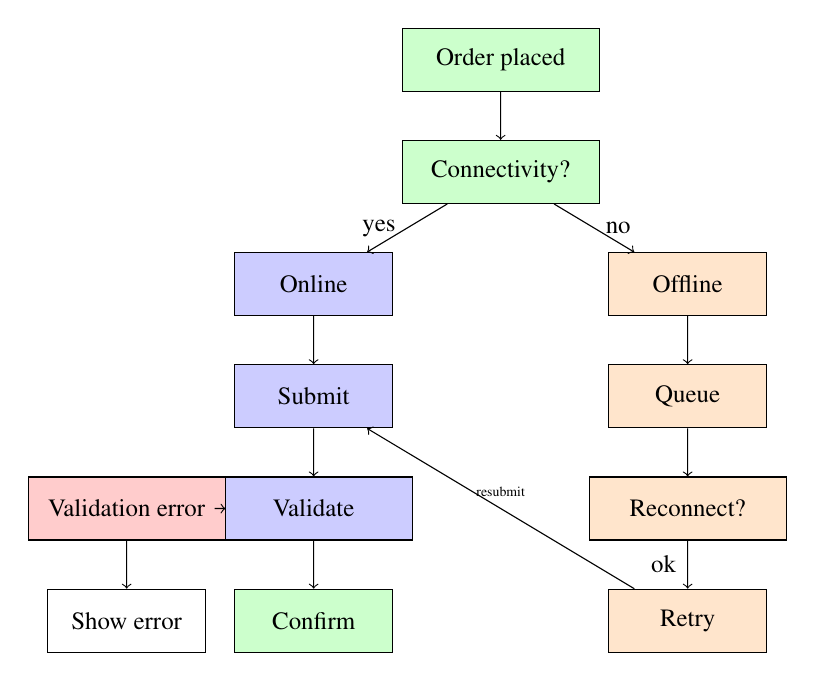
\begin{tikzpicture}[scale=0.95,every node/.style={font=\small}]

%Main flow
\node[draw,rectangle,minimum width=2.5cm,minimum height=0.8cm,fill=green!20] (order) at (1,8) {Order placed};
\node[draw,rectangle,minimum width=2.5cm,minimum height=0.8cm,fill=green!20] (check) at (1,6.5) {Connectivity?};

% Online path
\node[draw,rectangle,minimum width=2cm,minimum height=0.8cm,fill=blue!20] (online) at (-1.5,5) {Online};
\node[draw,rectangle,minimum width=2cm,minimum height=0.8cm,fill=blue!20] (submit) at (-1.5,3.5) {Submit};
\node[draw,rectangle,minimum width=2.5cm,minimum height=0.8cm,fill=blue!20] (validate) at (-1.5,2) {Validate};

% Online success
\node[draw,rectangle,minimum width=2cm,minimum height=0.8cm,fill=green!20] (success) at (-1.5,0.5) {Confirm};

% Online error
\node[draw,rectangle,minimum width=2.5cm,minimum height=0.8cm,fill=red!20] (online-err) at (-4,2) {Validation error};
\node[draw,rectangle,minimum width=2cm,minimum height=0.8cm] (show-err) at (-4,0.5) {Show error};

% Offline path
\node[draw,rectangle,minimum width=2cm,minimum height=0.8cm,fill=orange!20] (offline) at (3.5,5) {Offline};
\node[draw,rectangle,minimum width=2cm,minimum height=0.8cm,fill=orange!20] (queue) at (3.5,3.5) {Queue};
\node[draw,rectangle,minimum width=2.5cm,minimum height=0.8cm,fill=orange!20] (reconnect) at (3.5,2) {Reconnect?};
\node[draw,rectangle,minimum width=2cm,minimum height=0.8cm,fill=orange!20] (retry) at (3.5,0.5) {Retry};

% Connections
\draw[->] (order) -- (check);
\draw[->] (check) -- (online) node[midway,left] {yes};
\draw[->] (check) -- (offline) node[midway,right] {no};

\draw[->] (online) -- (submit);
\draw[->] (submit) -- (validate);
\draw[->] (validate) -- (success);
\draw[->] (validate) -- (online-err);
\draw[->] (online-err) -- (show-err);

\draw[->] (offline) -- (queue);
\draw[->] (queue) -- (reconnect);
\draw[->] (reconnect) -- (retry) node[midway,left] {ok};
\draw[->] (retry) -- (submit) node[midway,above,font=\tiny] {resubmit};

\end{tikzpicture}
\caption{Error handling and resilience: online operations validated immediately, offline operations queued and retried upon reconnection.}
\end{figure}

\subsection{Low-Level Design Diagrams (Explained in Text Form)}

Several design patterns detailed at implementation level provide concrete specificity.

\textbf{Data Model Design:} The database schema reflects denormalization decisions optimized for mobile query efficiency. A patient document in the Firestore users collection contains basic profile information (name, phone, address). Rather than storing patient appointment history as references and requiring a separate query to the appointments collection, a patient document maintains an array of appointment IDs embedded directly, allowing the patient's profile to display "upcoming appointments" with a single document read. This denormalization trades storage space for query efficiency—if a patient modifies their address, both the user document and all subsequent appointments include the updated address, requiring a write transaction across multiple documents. In SQL databases, such denormalization would be considered an anti-pattern; in NoSQL systems optimized for mobile access, this pattern is standard.

\textbf{Figure 3.3: Database Denormalization Pattern} shows how patient data is structured with embedded appointment references versus the traditional relational normalized approach. The embedded approach allows querying a single document for complete patient context; the normalized approach would require joins across multiple tables and multiple queries.

\begin{figure}[H]
\centering
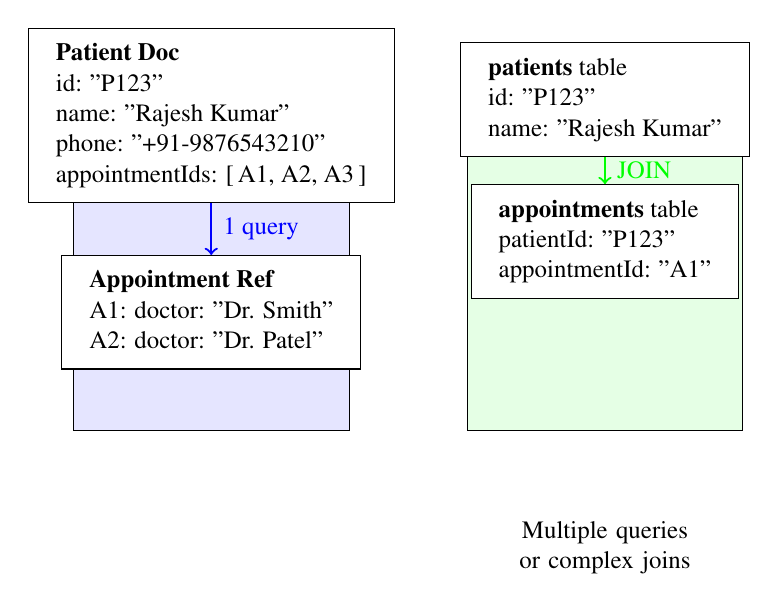
\begin{tikzpicture}[scale=1,every node/.style={font=\small}]

% Left side - Denormalized (recommended for NoSQL)
\node[draw,rectangle,minimum width=3.5cm,minimum height=4cm,fill=blue!10] (denorm) at (2.5,5) {};
\node[anchor=north,font=\bfseries] at (denorm.north) {Denormalized (NoSQL)};

\node[draw,rectangle,minimum width=3cm,minimum height=1.5cm,fill=white] (patient) at (2.5,7) {
  \begin{tabular}{l}
    \textbf{Patient Doc} \\
    id: "P123" \\
    name: "Rajesh Kumar" \\
    phone: "+91-9876543210" \\
    appointmentIds: [\,A1, A2, A3\,]
  \end{tabular}
};

\node[draw,rectangle,minimum width=3cm,minimum height=1.2cm,fill=white] (appt) at (2.5,4.5) {
  \begin{tabular}{l}
    \textbf{Appointment Ref} \\
    A1: {doctor: "Dr. Smith"} \\
    A2: {doctor: "Dr. Patel"}
  \end{tabular}
};

\draw[->,thick,blue] (patient) -- (appt) node[midway,right] {1 query};

% Right side - Normalized (traditional SQL)
\node[draw,rectangle,minimum width=3.5cm,minimum height=4cm,fill=green!10] (norm) at (7.5,5) {};
\node[anchor=north,font=\bfseries] at (norm.north) {Normalized (SQL)};

\node[draw,rectangle,minimum width=3cm,minimum height=1.2cm,fill=white] (normpatient) at (7.5,7.2) {
  \begin{tabular}{l}
    \textbf{patients} table \\
    id: "P123" \\
    name: "Rajesh Kumar"
  \end{tabular}
};

\node[draw,rectangle,minimum width=3cm,minimum height=1.2cm,fill=white] (normappt) at (7.5,5.4) {
  \begin{tabular}{l}
    \textbf{appointments} table \\
    patientId: "P123" \\
    appointmentId: "A1"
  \end{tabular}
};

\draw[->,thick,green] (normpatient) -- (normappt) node[midway,right] {JOIN};
\node[below=1cm of norm,font=\small,text width=3cm,text centered] {Multiple queries or complex joins};

\end{tikzpicture}
\caption{Denormalization strategy for NoSQL: patient documents embed appointment IDs for single-query access versus normalized SQL requiring joins.}
\end{figure}

\textbf{Real-Time Location Update Pattern:} The delivery tracking feature implements a pub-sub messaging pattern where delivery devices publish location coordinates and client apps subscribe to receive updates. Rather than apps polling ("is there new location data?") every second, the backend pushes updates to subscribed clients. Firebase Realtime Database listeners implement this pattern—the app registers a listener for the specific delivery's location collection, and Firestore invokes the listener callback whenever new data arrives. This push-based approach reduces battery consumption (no polling overhead) and provides lower latency (updates arrive immediately rather than after polling delay).

\textbf{Authentication and Authorization Pattern:} The system implements JWT (JSON Web Token) authentication where Firebase Authentication issues tokens that include user role and identifier. The client app stores this token in encrypted SharedPreferences (Android secure storage). For every API call, the app includes the token in the HTTP Authorization header. Cloud Functions verify the token's validity and extract user information. Firestore security rules similarly access token information through context.auth properties, enabling rules like "allow read if document.patientID == request.auth.uid"—this rule permits a user to read a document only if the document's patientID field matches their authenticated user ID.

\textbf{Figure 3.4: Authentication and Authorization Flow} shows how tokens move through the system. A user logs in through Firebase Authentication; the system returns a JWT token. The app stores this token securely and includes it in every subsequent request. The backend verifies the token and uses embedded user information to enforce access control at multiple layers (Cloud Functions check permissions, Firestore rules verify document-level access).

\begin{figure}[H]
\centering
\begin{tikzpicture}[scale=0.95]
\node[draw,rectangle,minimum width=1.5cm] (user) at (0.75,8) {User};
\node[draw,rectangle,minimum width=1.5cm] (app) at (3,8) {Mobile\\App};
\node[draw,rectangle,minimum width=1.5cm] (auth) at (5.25,8) {Firebase\\Auth};
\node[draw,rectangle,minimum width=1.5cm] (cloud) at (7.5,8) {Cloud\\Function};
\node[draw,rectangle,minimum width=1.5cm] (db) at (9.75,8) {Firestore};

% Lifelines
\foreach \node in {user,app,auth,cloud,db} {
  \draw[dashed] (\node) -- (\node|-0.5);
}

% Step 1: User provides credentials
\draw[->,thick] (user) -- (app) node[midway,above,font=\tiny] {credentials};

% Step 2: App sends to Firebase
\draw[->,thick] (app) -- (auth) node[midway,above,font=\tiny] {email+password};

% Step 3: Firebase returns JWT
\draw[->,thick] (auth) -- (app) node[midway,above,font=\tiny] {JWT token};

% Step 4: App stores and uses token
\node[fill=yellow!20] (store) at (3,-0.3) {\small token in\\SharedPreferences};
\draw[->] (app) -- (store);

% Step 5: App includes token in request
\draw[->,thick] (app) -- (cloud) node[midway,above,font=\tiny] {request+token};

% Step 6: Cloud verifies and checks
\draw[->,thick] (cloud) -- (db) node[midway,above,font=\tiny] {verify token\\for access};

% Step 7: Response with authorization
\draw[->,thick] (db) -- (cloud) node[midway,above,font=\tiny] {data if auth};

% Step 8: Back to app
\draw[->,thick] (cloud) -- (app) node[midway,above,font=\tiny] {response};

\end{tikzpicture}
\caption{JWT-based authentication flow where tokens are issued by Firebase, stored securely on the device, and verified at each access layer.}
\end{figure}

\textbf{Consistency and Transaction Management:} Appointment booking requires consistency guarantees—the same appointment slot cannot be booked by two patients simultaneously. Firestore handles this through transactions. When a patient books a slot, the client submits a transaction request that atomically: (1) increments the booking counter for that slot, (2) checks whether the counter now exceeds maximum capacity, (3) if capacity violated, aborts the transaction and rolls back the counter; (4) if capacity available, creates the appointment document. Any other concurrent booking attempt attempting the same slot will see the transaction already in progress and must wait or accept conflict. This optimistic locking approach handles concurrency without requiring explicit locks that could deadlock.

\textbf{Caching Strategy:} The app implements a three-tier caching strategy. First, in-memory caches in ViewModels hold frequently accessed data (current appointments, current orders) for 5 minutes. Second, local Room database caches persist across app restarts—prescriptions, appointments, and historical orders are cached locally. Third, Firestore implements server-side caching through the free tier's offline support; client libraries maintain a local cache of queries and serve queries from cache when offline. This multi-layer caching optimizes both latency (most queries serve from memory or local database within 50 milliseconds) and reliability (offline operation possible within cached data scope).

\textbf{Figure 3.5: Three-Tier Caching Architecture} illustrates the caching hierarchy. In-memory caches serve the fastest responses but have shortest lifetime. Room database caches persist across app sessions but have slight latency overhead from local database reads. Firestore client library caching enables offline operation when network is unavailable.

\begin{figure}[H]
\centering
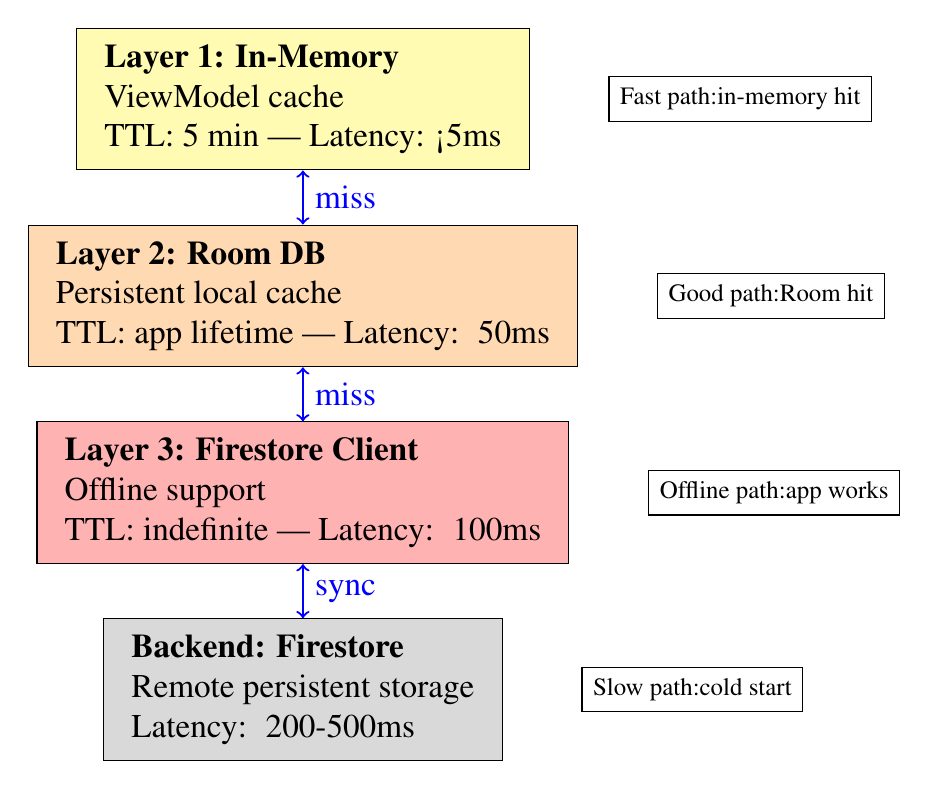
\begin{tikzpicture}[scale=1]

% Layer 1: In-memory
\node[draw,rectangle,minimum width=3.5cm,minimum height=1.5cm,fill=yellow!30] (l1) at (2.5,8) {
  \begin{tabular}{l}
    \textbf{Layer 1: In-Memory} \\
    ViewModel cache \\
    TTL: 5 min | Latency: <5ms
  \end{tabular}
};

% Layer 2: Room Database
\node[draw,rectangle,minimum width=3.5cm,minimum height=1.5cm,fill=orange!30] (l2) at (2.5,5.5) {
  \begin{tabular}{l}
    \textbf{Layer 2: Room DB} \\
    Persistent local cache \\
    TTL: app lifetime | Latency: ~50ms
  \end{tabular}
};

% Layer 3: Firestore Client Cache
\node[draw,rectangle,minimum width=3.5cm,minimum height=1.5cm,fill=red!30] (l3) at (2.5,3) {
  \begin{tabular}{l}
    \textbf{Layer 3: Firestore Client} \\
    Offline support \\
    TTL: indefinite | Latency: ~100ms
  \end{tabular}
};

% Backend
\node[draw,rectangle,minimum width=3.5cm,minimum height=1.5cm,fill=gray!30] (backend) at (2.5,0.5) {
  \begin{tabular}{l}
    \textbf{Backend: Firestore} \\
    Remote persistent storage \\
    Latency: ~200-500ms
  \end{tabular}
};

% Arrows showing relationships
\draw[<->,thick,blue] (l1) -- (l2) node[midway,right] {miss};
\draw[<->,thick,blue] (l2) -- (l3) node[midway,right] {miss};
\draw[<->,thick,blue] (l3) -- (backend) node[midway,right] {sync};

% Path example
\node[right=1cm of l1,font=\small,draw,rectangle,align=center] {Fast path:\newline in-memory hit};
\node[right=1cm of l2,font=\small,draw,rectangle,align=center] {Good path:\newline Room hit};
\node[right=1cm of l3,font=\small,draw,rectangle,align=center] {Offline path:\newline app works};
\node[right=1cm of backend,font=\small,draw,rectangle,align=center] {Slow path:\newline cold start};

\end{tikzpicture}
\caption{Three-tier caching hierarchy reducing latency through memory, persisted local database, and offline support.}
\end{figure}

MediTrack's architecture represents pragmatic choices balancing engineering effort, operational complexity, and user experience. Using managed services (Firebase) rather than building custom infrastructure traded some flexibility for rapid development. Implementing offline-first design traded simplicity for resilience given India's variable network conditions. Denormalizing data traded consistency complexity for mobile query efficiency. These trade-offs were deliberate—the team evaluated alternative architectures and consciously chose this approach as optimal given constraints.

\section*{CHAPTER SUMMARY}

System analysis establishes the what, who, how, and why of MediTrack's design. The overall system description identifies MediTrack as a coordination layer integrating three previously disconnected healthcare workflows (appointment scheduling, prescription fulfillment, delivery logistics) without attempting to replace the entire healthcare system. The system must function across diverse hardware (budget Android devices), variable network conditions (ranging from 4G urban to 2G rural), and battery-constrained devices.

User classes—patients, healthcare providers, and pharmacy staff—interact with the system through different patterns. Patients access appointments and track deliveries episodically. Providers use the system during patient interactions. Pharmacy staff access the system continuously during their operational day. System design must accommodate all three usage patterns simultaneously.

Functional requirements specify concrete capabilities the system must provide: appointment management, prescription recording, order placement, real-time delivery tracking, and granular notification control. Non-functional requirements define quality attributes: responses must complete in under 2 seconds, the system must maintain 99 percent uptime, all communication must use TLS 1.2 encryption, and interfaces must be usable by non-technical users.

The architecture implementing these requirements divides into layers: presentation (Android app with MVVM pattern), network communication (Firebase SDKs abstracting HTTP), backend services (Cloud Functions handling validation and payment), database (Firestore providing real-time synchronization), and external integrations (Maps, payment processors). This architecture trades some flexibility for operational simplicity through managed services, handles offline scenarios through local caching, and enforces security through database-layer access rules rather than relying on application validation.

\end{document}
